\documentclass{beamer}
\mode<presentation>
\usepackage{amsmath}
\usepackage{amssymb}
\usepackage{adjustbox}
\usepackage{subcaption}
\usepackage{enumitem}
\usepackage{multicol}
\usepackage{mathtools}
\usepackage{listings}
\usepackage{url}
\def\UrlBreaks{\do\/\do-}
\usetheme{Boadilla}
\usecolortheme{lily}
\setbeamertemplate{footline}


% Code style
\lstset{
  basicstyle=\ttfamily\scriptsize,
  breaklines=true,
  frame=single,
  numbers=left,
  numberstyle=\tiny,
  keywordstyle=\color{blue},
  commentstyle=\color{green!50!black},
  stringstyle=\color{red!60!black},
  showstringspaces=false
}

{
  \leavevmode%
  \hbox{%
  \begin{beamercolorbox}[wd=\paperwidth,ht=2.25ex,dp=1ex,right]{author in head/foot}%
    \insertframenumber{} / \inserttotalframenumber\hspace*{2ex} 
  \end{beamercolorbox}}%
  \vskip0pt%
}
\setbeamertemplate{navigation symbols}{}

\title{1.2.23 -- Matgeo Assignment}
\author{ai25btech11015 -- M Sai Rithik}
\date{}

\begin{document}
\frame{\titlepage}

%------------------------------------------------
\begin{frame}{Question}
Represent graphically a displacement of \(\,40\,\text{km},\;30^\circ\) west of south.
\end{frame}

%------------------------------------------------
\begin{frame}{Coordinate Convention}
We choose the coordinate axes as:
\[
\text{East} \equiv +x,\quad
\text{West} \equiv -x,\quad
\text{North} \equiv +y,\quad
\text{South} \equiv -y.
\]

The unit column for South is
\[
\mathbf{s} = 
\begin{bmatrix}
0 \\ -1
\end{bmatrix}.
\]
\end{frame}

%------------------------------------------------
\begin{frame}{Rotation Matrix}
For rotation by angle \(\theta\) anti clockwise,
\[
R(\theta) =
\begin{bmatrix}
\cos\theta & -\sin\theta\\
\sin\theta & \cos\theta
\end{bmatrix}.
\]

Since “\(30^\circ\) west of south” means clockwise rotation of \(30^\circ\) or anti-clockwise roation of \(330^\circ\),we apply
\[
\mathbf{u} = R(330^\circ)\mathbf{s}.
\]
\end{frame}

%------------------------------------------------
\begin{frame}{Direction Column}
\[
\mathbf{u} =
\begin{bmatrix}
\cos 330^\circ & \;\;-\sin 330^\circ \\
\sin 330^\circ & \cos 330^\circ
\end{bmatrix}
\begin{bmatrix}
0 \\ -1
\end{bmatrix}
=
\begin{bmatrix}
-\tfrac{1}{2}\\[4pt]
-\tfrac{\sqrt{3}}{2}
\end{bmatrix}.
\]
\end{frame}

%------------------------------------------------
\begin{frame}{Displacement Column}
With magnitude \(40\) km:
\[
\mathbf{d} = 40\mathbf{u}
= 40
\begin{bmatrix}
-\tfrac{1}{2}\\[2pt]
-\tfrac{\sqrt{3}}{2}
\end{bmatrix}
=
\begin{bmatrix}
-20\\[2pt]
-20\sqrt{3}
\end{bmatrix}\;\text{km}.
\]

Endpoint:
\[
(x,y) = (-20,\; -20\sqrt{3}) \;\text{km}.
\]
\end{frame}

%------------------------------------------------
\begin{frame}{Graphical Representation}
\begin{figure}[h!]
    \centering
    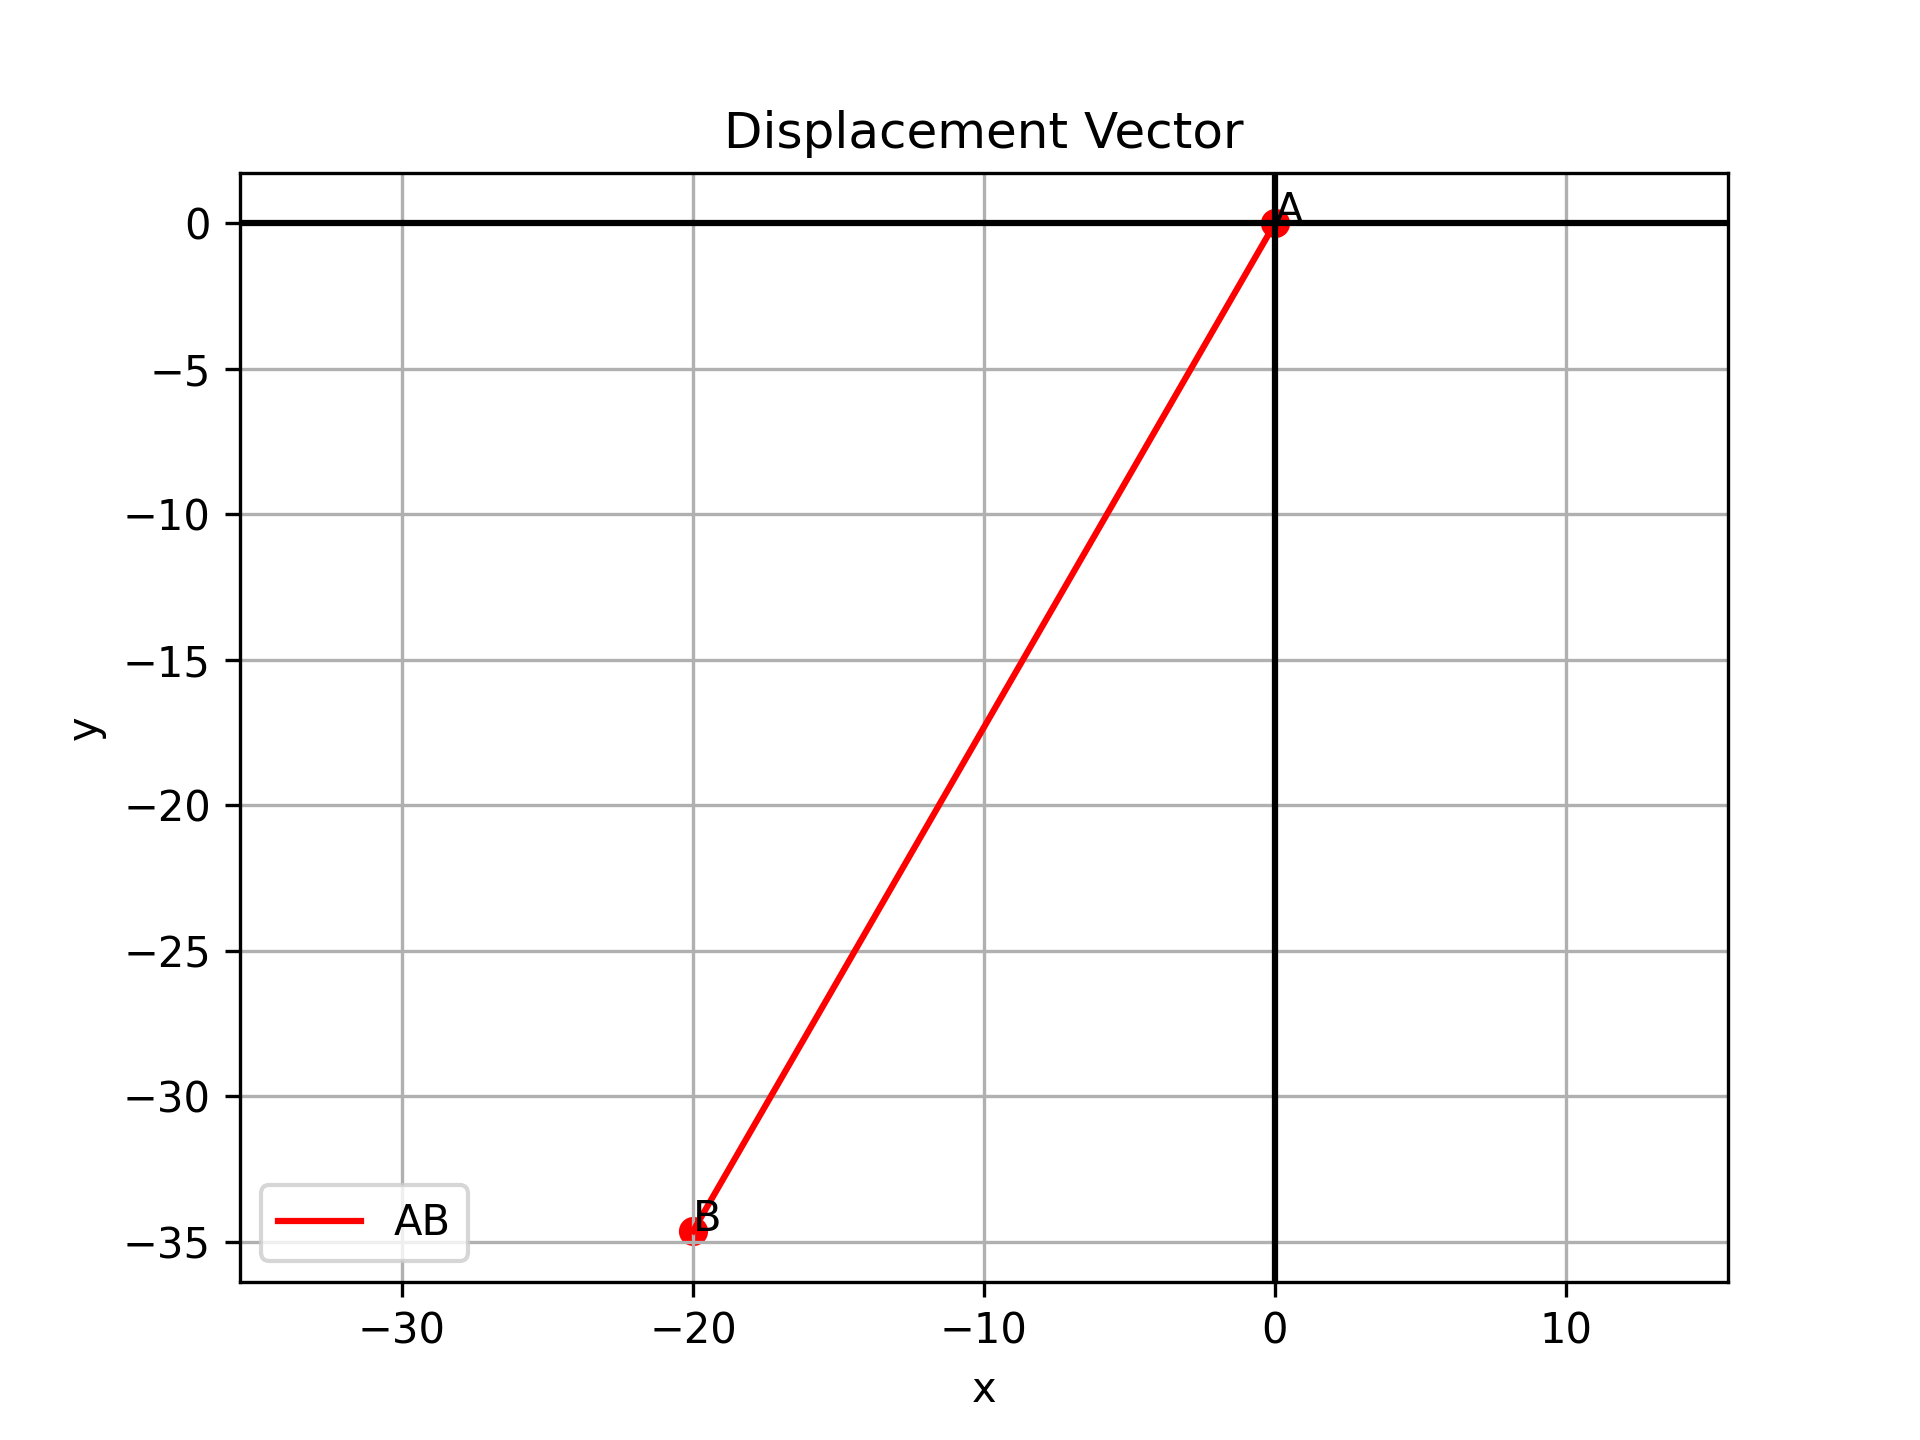
\includegraphics[width=0.65\linewidth]{figs/fig.png}
    \caption{Displacement vector: 40 km, \(30^\circ\) west of south}
\end{figure}
\end{frame}

% -------- C Code Split Across Frames ----------
\begin{frame}[fragile]
    \frametitle{C Code}
    \begin{lstlisting}[language=C]
#include <stdio.h>
#include <stdlib.h>
#include <math.h>
#include "libs/matfun.h"

int main() {

    /* This code calculates 30 degrees west of south */
    
    // Create 2x2 rotation matrix
    double **R = rotMat(-M_PI/6);
    // Create 2x1 south vector (column vector)
    double **v = createMat(2, 1);
    v[0][0] = 0;
    v[1][0] = -1;

    // Multiply: (2x2) * (2x1) = (2x1)
    double **rotated = Matmul(R, v, 2, 2, 1);

    // Print result
    printf("Rotated vector: (%.4f, %.4f)\n", rotated[0][0], rotated[1][0]);
    
    \end{lstlisting}
\end{frame}

\begin{frame}[fragile]
    \frametitle{C Code}
    \begin{lstlisting}[language=C]
    FILE *fp = fopen("var.dat", "w");
    if (fp != NULL) {
        fprintf(fp, "%.4f\n%.4f\n", rotated[0][0], rotated[1][0]);
        fclose(fp);
    } else {
        printf("Error opening file for writing.\n");
    }
    
    return 0;
}

    \end{lstlisting}
\end{frame}

\begin{frame}[fragile]
    \frametitle{Python Code}
    \begin{lstlisting}[language=Python]

import matplotlib.pyplot as plt
import numpy as np 
# Code by M SAI RITHIK
# 1.2.23 Represent graphically a displacement
# of 40 km, 30◦ west of south.
# (−20, −20 √3)

coords = np.loadtxt('var.dat', delimiter=' ')
point = np.array(coords) * 40


origin = np.array([0,0])

vec = np.array([origin,point])


plt.plot(vec[:,0], vec[:,1], color="red",label="AB")
plt.scatter(vec[:,0], vec[:,1],color = "red")
plt.title("Displacement Vector")

plt.text(vec[0,0],vec[0,1],"A")
plt.text(vec[1,0],vec[1,1],"B")
\end{lstlisting}
\end{frame}



\begin{frame}[fragile]
    \frametitle{Python Code}
    \begin{lstlisting}[language=Python]

plt.axhline(0, color='black')   # x-axis
plt.axvline(0, color='black')   # y-axis
plt.xlabel("x")
plt.ylabel("y")
plt.grid(True)
plt.axis("equal")
plt.legend(loc="best")
plt.show()
plt.savefig('../figs/fig.png', dpi=300)

    \end{lstlisting}
\end{frame}

\end{document}

% \documentclass{beamer}
% \usetheme{Madrid}

% \usepackage{amsmath, amssymb, amsthm}
% \usepackage{graphicx}
% \usepackage{gensymb}
% \usepackage[utf8]{inputenc}
% \usepackage{hyperref}
% \usepackage{tikz}

% \title{1.2.23 Matgeo}
% \author{AI25BTECH11015 - M Sai Rithik}
% \date{}

% \begin{document}

% \frame{\titlepage}

% % Question frame
% \begin{frame}
% \frametitle{Question}
% Represent graphically a displacement of 40 km, $30^{\circ}$ west of south.
% \end{frame}

% % Coordinate system assumptions
% \begin{frame}
% \frametitle{Coordinate System}
% We choose the coordinate axes such that:
% \begin{itemize}
%     \item $+x$ axis $\to$ East
%     \item $+y$ axis $\to$ North
% \end{itemize}
% \end{frame}

% % Solution steps
% \begin{frame}
% \frametitle{Solution}
% The given displacement has magnitude
% \[
% |\vec{D}| = 40 \ \text{km}
% \]
% and direction $30^{\circ}$ west of south.  

% \[
% \theta = 270^{\circ} - 30^{\circ} = 240^{\circ}.
% \]
% \end{frame}

% \begin{frame}
% \frametitle{Vector Components}
% The vector components are:
% \[
% D_x = 40 \cos 240^{\circ} = -20,
% \]
% \[
% D_y = 40 \sin 240^{\circ} = -20\sqrt{3}.
% \]

% Therefore,
% \[
% \vec{D} = -20\hat{i} - 20\sqrt{3}\hat{j}.
% \]
% \end{frame}

% % Graphical representation
% \begin{frame}
% \frametitle{Graphical Representation}
% The displacement vector is drawn from $(0,0)$ to:
% \[
% (-20, \ -20\sqrt{3}).
% \]

% \begin{center}
% 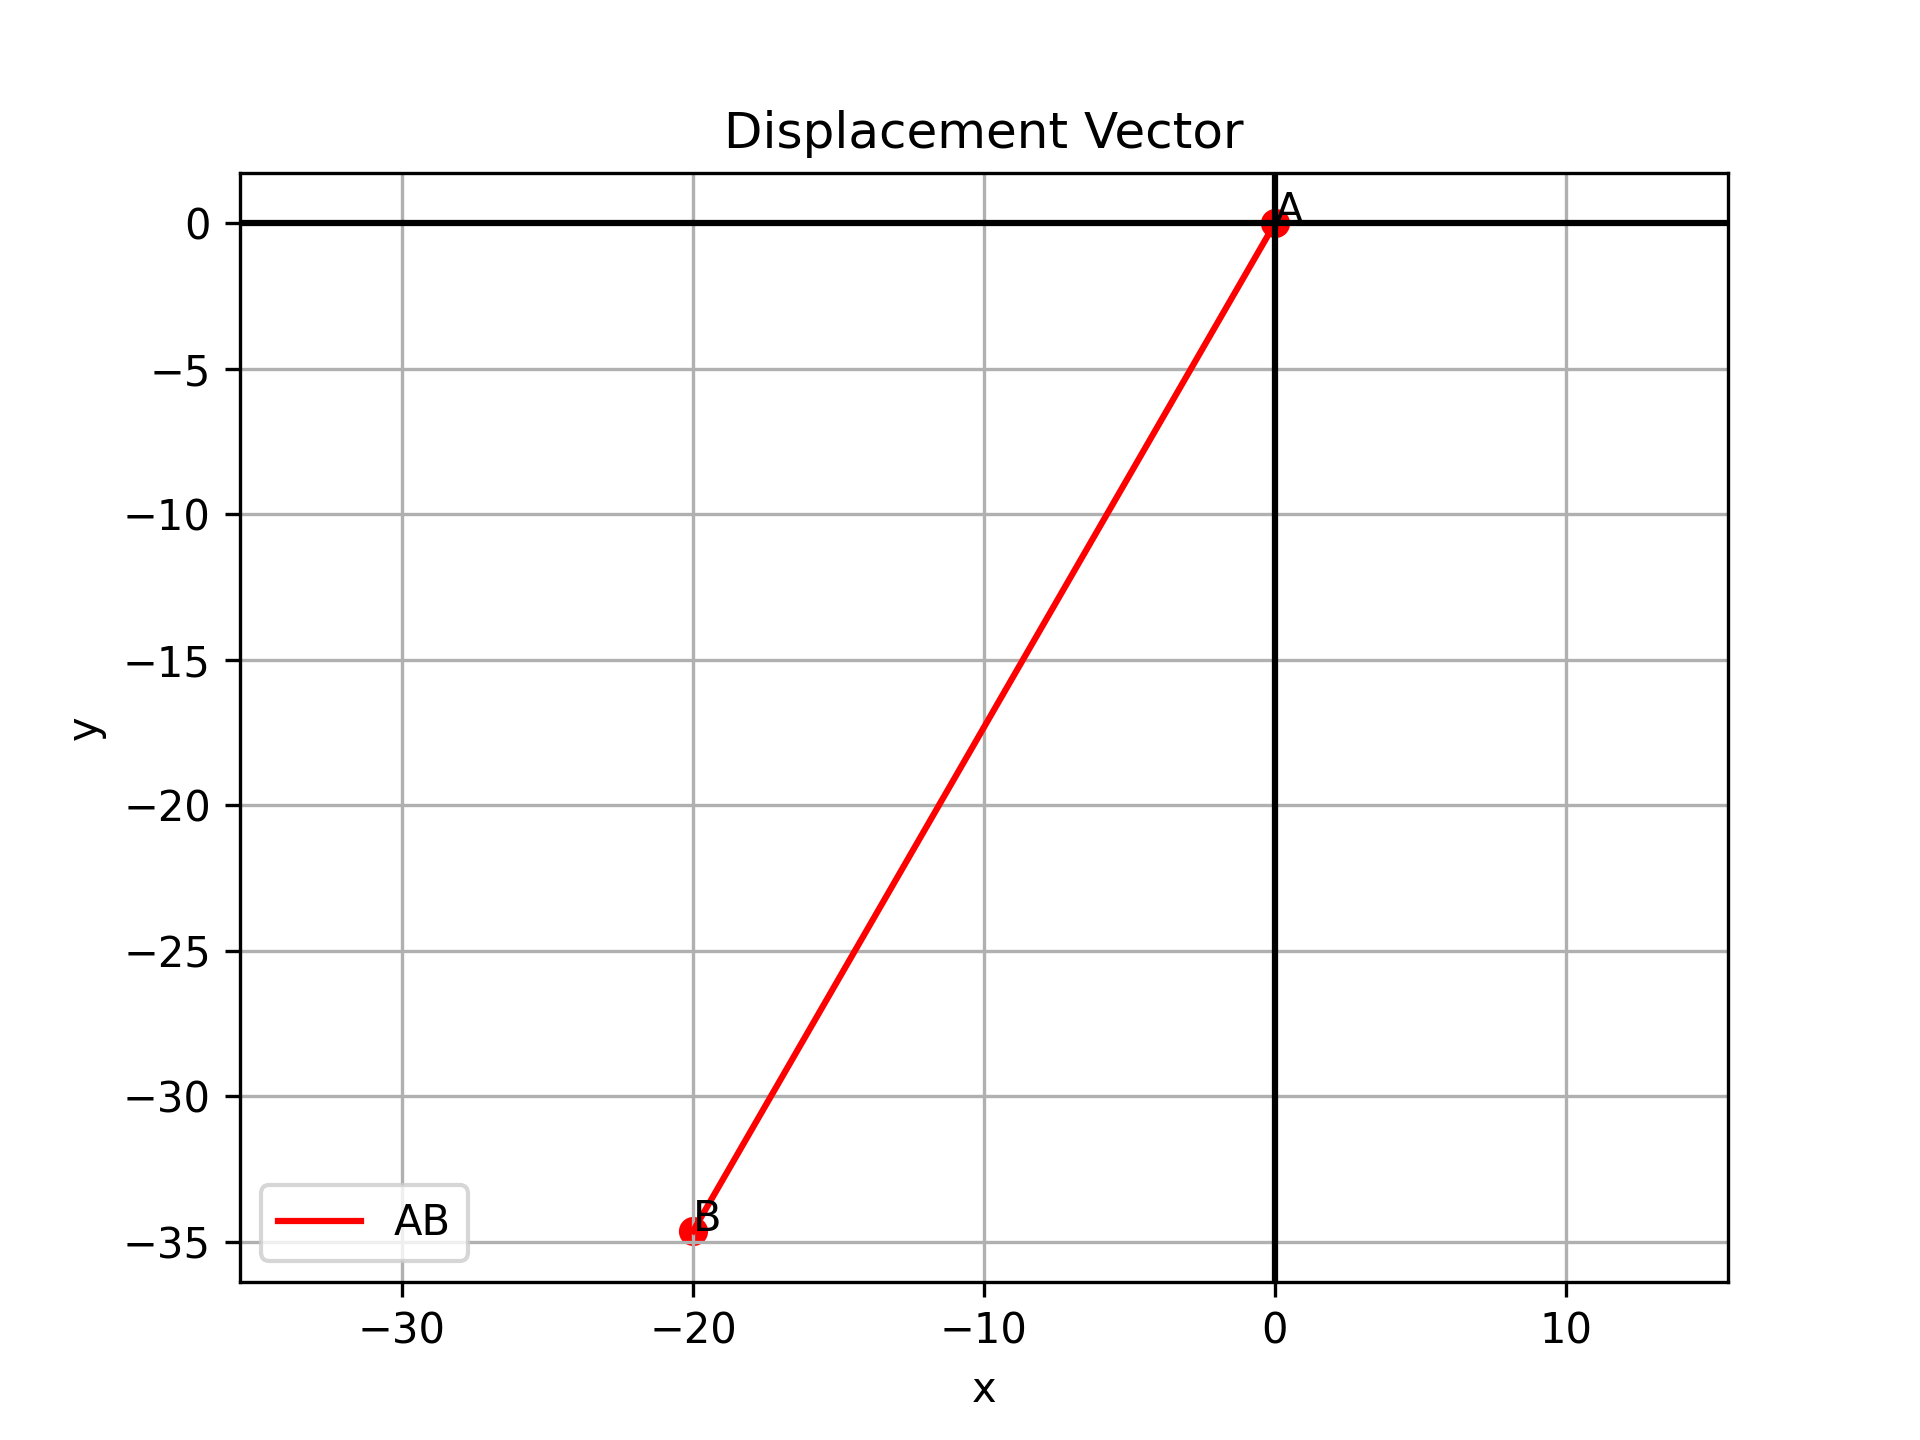
\includegraphics[width=0.6\linewidth]{figs/fig.png}
% \end{center}
% \end{frame}

% \end{document}
